\chapter{Mezuro: Uma plataforma de Monitoramento de Código Fonte}

%Introdução
A prática da engenharia de software exige compreensão do projeto como um todo, onde o código-fonte é uma das partes mais importantes. O engenheiro de software precisa analizar um código-fonte diversas vezes, seja para desenvolver novas funcionalidades ou melhorar as existentes \cite{meirelles2010mezuro}.

Como parte fundamental do projeto de software, o código-fonte é um dos principais artefatos para avaliar sua qualidade \cite{meirelles2009crab}. Essas avaliações não são meramente subjetivas, sendo necessário extrair informações que possam ser replicadas e entendidas da mesma forma, independente de quem analisa o código. As métricas de código-fonte permitem esse tipo de avaliação pois possibilitam analisar, de forma objetiva, as principais características para aceitação de um software.

%Métricas código-fonte
Há várias características que fazem do software um sistema de qualidade ou não. Entre elas há algumas que são obtidas exclusivamente através do código-fonte. Quando compilamos um software, por exemplo, características podem ser analisadas, mas outras como organização e legibilidade não. Isso não refletiria tamanho, modularidade, manutenbilidade, complexidade, flexibilidade, que são características encontradas na análise de códigos-fonte \cite{meirelles2013metrics}.

%Ferramentas para monitoramento de métricas de código-fonte
Extrair métricas de um código-fonte manualmente, é uma tarefa bastante difícil, independente do tamanho do código. Porém quanto maior e mais complexo é o código, essa tarefa se torna praticamente impossível pela quantidade de atributos e linhas de códigos a se analisar, além de não ser viável pelo tempo despendido nessa tarefa. Por outro lado há ferramentas CASE para monitoramento automático de códigos-fonte. Para isso existem poucas ferramentas disponíveis no mercado, e muitas delas nem sempre são adequadas para análise do projeto alvo (software-livre) \cite{meirelles2010mezuro}.
%Métricas são fundamentais para a melhora contínua de um projeto de software livre

%Mezuro
  %Histórico Ferramentas até chegar ao Mezuro [tese prof. Paulo] 
    %Contexto das ferramentas
A partir da necessidade de extrair métricas de código-fonte e interpretar seus valores possibilitando o monitoramento de características específicas do software foi desenvolvida uma plataforma chamada Mezuro \cite{meirelles2010mezuro}. O Mezuro porém não foi criado da noite para o dia. Ele foi concebido através de um longo processo de amadurecimento de diversas ferramentas, que teve seu início com o projeto Qualipso.

\section{O Projeto Qualipso}

	%Projeto Qualipso
O projeto (Qualipso Quality Platform for Open Source) é hoje um consórcio formado por indústria, academia, e governo. Seu principal objetivo é potencializar as práticas de desenvolvimento de software livre, tornando-as confiáveis, reconhecidas e estabelecidas na indústria, através da implementação de tecnologias, procedimentos e leis \cite{qualipso2009}. 
	
	%Jabuti, ponto de partida
Uma das iniciativas desse projeto envolvia  a adaptaçao da ferramenta JaBUTi - Java Bytecode Understanding and Testing, uma ferramenta de análise de softwares em linguagem Java. O objetivo inicial era melhorar o módulo de cálculo das métricas fornecido pela JaBUTi. Porém a proposta foi alterada para a visualização de métricas, com configuração de intervalos das mesmas, facilitando a análise dos resultados. Esse módulo de visualização, posteriormente, se transformou em uma aplicação independente, o Crab \cite{meirelles2009crab}. Neste instante o JaBUTi calculava asa métricas então chamava o Crab para visualiza-las, assim como possibilitar configurações e criação de métricas compostas. Após a experiência com a JaBUTi como ferramenta base, ou seja, aquela que coleta métricas de código-fonte, buscou-se outras alternativas para essa tarefa já que a JaBUTi era restrita a códigos escritos  em liguagem Java, o que limita a contribuição com softwares livre.

	%Analizo
Uma alternativa encontrada foi o software livre denominado Analizo, o qual surgiu a partir de um outro software livre denominado Egypt. Após diversas contribuições (principalemnte de Antônio Terceiro e do grupo CCSL-USP) resultou em diversas funcionalidades que fugiram do escopo inicial do Egypt, que passou a ser o Analizo, "análise" em esperanto. 

Na integração do Analizo com a Crab, a Crab consome, requisita serviços do Analizo, ao contrário do que acontecia na integração da JaBUTi com a Crab, onde a ferramenta base aciona o módulo de visualização (Crab) após a coleta das métricas.

%----------------------------------------------------------------------------%

\section{Mezuro como Plugin do Noosfero}

%O que é o Noosfero
O Mezuro foi concebido como instância de uma plataforma web conhecida como Noosfero com o plugin Mezuro ativado. O Noosfero é um software livre para criação de redes sociais desenvolvido pela Cooperativa de Tecnologias Livres - Coolivre sob licença AGPL v.3 com o intuito de permitir com que os usuários criem sua própria rede social livre e personalizada de acordo com suas necessidades.

%Arquitetura do Noosfero
A linguagem de programação Ruby versão 1.8.7 e o framework MVC Ruby on Rails foram utilizados para desenvolver o Noosfero. Essas tecnologias foram escolhidas pois a linguagem Ruby possui uma sintaxe simples, que facilita a manunbilidade do sistema, característica importante em projetos de software livre que tendem a atrair colaboradores externos a equipe. Já o framework Ruby on Rails influencia em maior produtividade graças a conceitos como \textit{convention over configuration} e DRY [baseado TCC Daniel].

%Arquitetura de plugins do Noosfero
A arquitetura do Noosfero permite a adição de novas funcionalidades através de plugins. Essa característica é interessante pois colaboradores podem implementar novas funcionalidades sem entender ou interagir com o código-fonte do Noosfero, já que os plugins possuem o código isolado, mantendo o baixo acoplamento e alta coesão dos módulos do sistema. Embora plugins sejam totalmente independentes do sistema alvo, no Noosfero os plugins são mantidos com o código principal para auxiliar no controle de qualidade do ambiente. Pensando nisso os plugins devem ter testes automatizados para quando houver a necessidade de alterar o código do Noosfero, os testes dos plugins devem ser executados para verificar se as mudanças não afetaram seu funcionamento \cite{noosfero2013plugins}.

\graphicspath{{figuras/}}
\begin{figure}[!htb]
\centering
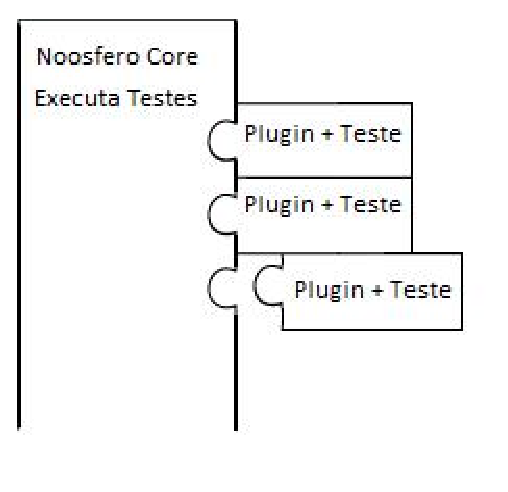
\includegraphics{plugins}
\caption{Arquitetura de Plugins do Noosfero}
\label{Rotulo}
\end{figure}

%Implementação do Mezuro como plugin do Noosfero
%Funcionalidades atuais do Mezuro
O Mezuro como plugin do Noosfero foi construído utilizando o recurso de plugins do framework Ruby on Rails. Por esse motivo ele herda a arquitetura desse framework, a qual é baseada no padrão arquitetural MVC, assim como o Noosfero.
O Mezuro utiliza um web service chamado Kalibro Metrics. Isso permite ao Mezuro: 

\begin{itemize}
\item Baixa códigos-fonte de repositórios dos tipos GIT, Subversion, Baazar e CVS
\item Criação de configuraçções as quais são conjuntos pré-definidos de métricas relacionadas para serem utilizadas na avaliação de projetos de software.
\item Criação de intervalos relacionados com a métricas e avaliações qualitativas.
\item Criação de novas métricas de acordo com aquelas fornecidas pelos coletores do Kalibro.
\item Cálculo de resultados estatísticos para módulos com alta granularidade.
\item Possibilidade de exportar arquivos com os resultados gerados.
\item Interpretação dos resultados com inteface mais amigável aos usuarios com a utilização de cores nos intervalos das métricas.
\end{itemize}



%----------------------------------------------------------------------------%

\section{Mezuro como aplicação independente}

%Motivos para evolução
  %Evolução do framework rails
  %Recursos desnecessários do Noosfero para o Mezuro
  
%Nova arquitetura
%Consumo dos serviços do Kalibro - webService
%Kalibro